\chapter{Effects of Variation on the Evolution of Larval Trait Parameters}
The stochasticity in the model comes from the initial variation in the larval trait parameters, given as certain variation in the respective initial distribution as well as from the heritability of the mid-parent value during the inheritance of the larval trait parameters. The simulations show how these sources of variations play an important role in determining the evolutionary routes taken to achieve greater competitive ability by having maximum survivorship.
\section{Variation in the Initial Distribution of Larval Trait Parameters}
In the initial distributions of all trait values, the variotion comes from the standard deviation given for each distribution. After $50^{th}$ generation, the initial standing variation in these trait distributions determine the maximum mean trait value that can be achieved to increase the fitness. Simulations were performed fro given fixed mean trait values but varying their respective initial standing variation to see how these variations interact to obtain maximum fitness in multiple ways. From fig~\ref{fig:ivar_fr_eff} - ~\ref{fig:ivar_mc_eff}, it is clear that differences in variation of these trait values, mean trait values at $50^{th}$ generation are different for different combinations of intial variation in trait values.\\\\

\begin{figure}[p]
  \subfloat{
  \centering
  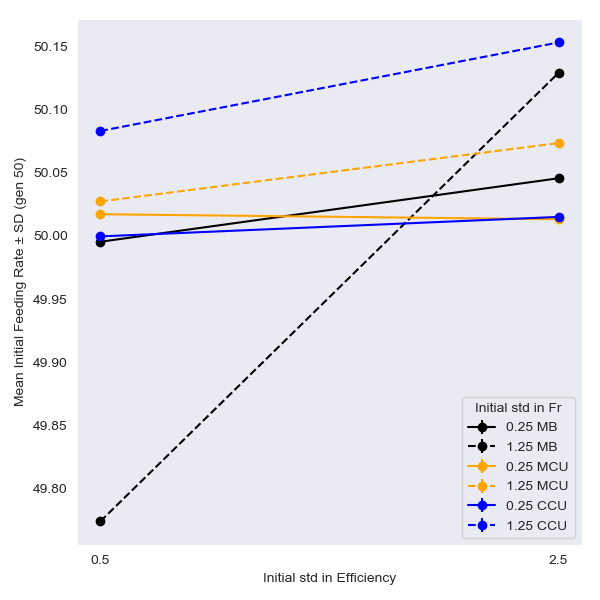
\includegraphics[width=0.5\textwidth]{C5/Figs/ivar/fr_eff_fr50}
  }
  \subfloat{
  \centering
  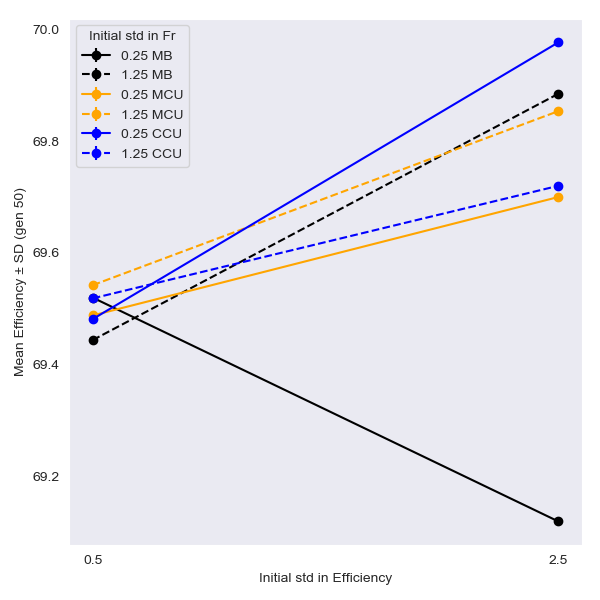
\includegraphics[width=0.5\textwidth]{C5/Figs/ivar/fr_eff_eff50}
  }
  \caption{Effect of initial variation in initial feeding rate and efficiency on mean trait values at generation 50.}
  \label{fig:ivar_fr_eff}
\end{figure}
\begin{figure}[p]
  \subfloat{
  \centering
  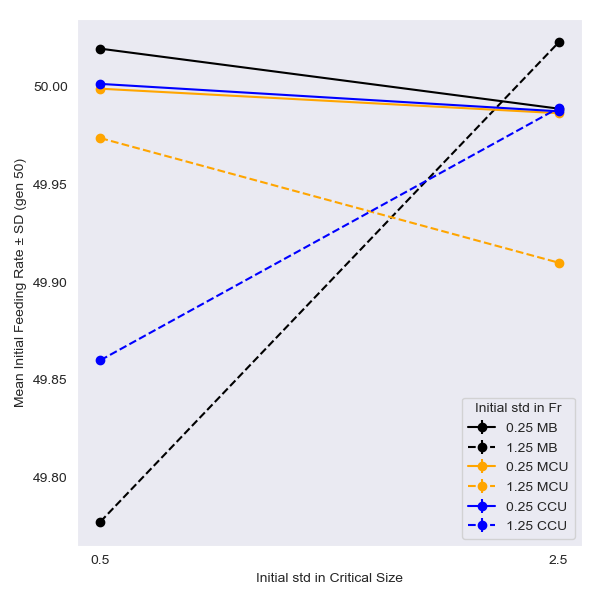
\includegraphics[width=0.5\textwidth]{C5/Figs/ivar/fr_mc_fr50}
  }
  \subfloat{
  \centering
  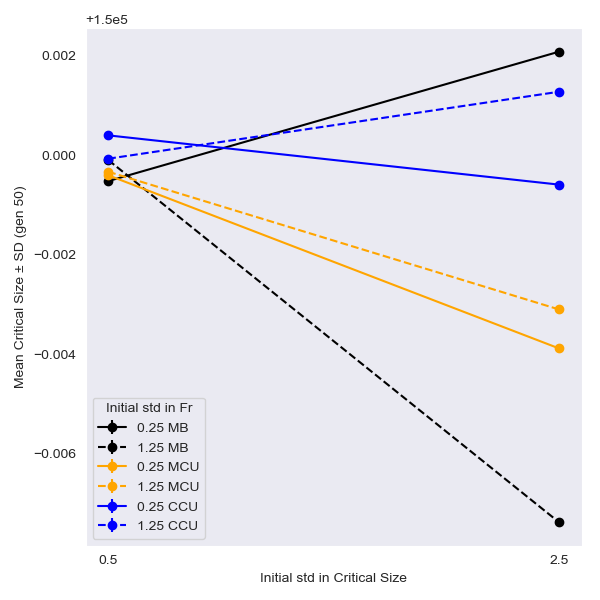
\includegraphics[width=0.5\textwidth]{C5/Figs/ivar/fr_mc_mc50}
  }
  \caption{Effect of initial variation in initial feeding rate and critical size on mean trait values at generation 50.}
  \label{fig:ivar_fr_mc}
\end{figure}
\begin{figure}[p]
  \subfloat{
  \centering
  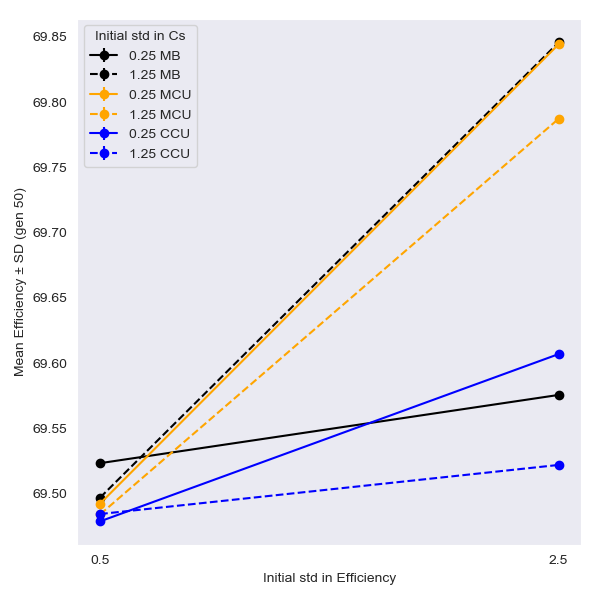
\includegraphics[width=0.5\textwidth]{C5/Figs/ivar/mc_eff_eff50}
  }\\
  \subfloat{
  \centering
  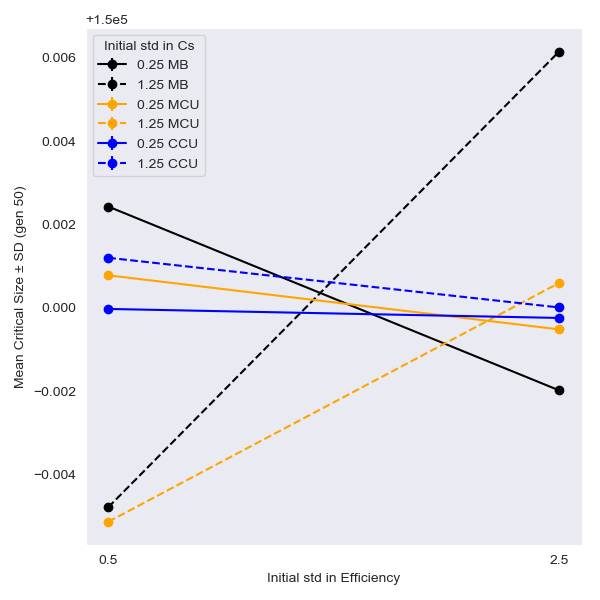
\includegraphics[width=0.5\textwidth]{C5/Figs/ivar/mc_eff_mc50}
  }
  \caption{Effect of initial variation in critical size and efficiency on mean trait values at generation 50.}
  \label{fig:ivar_mc_eff}
\end{figure}

\newpage
\section{Heritability of Mid-parent Value}
\begin{figure}[h]
  \subfloat{
  \centering
  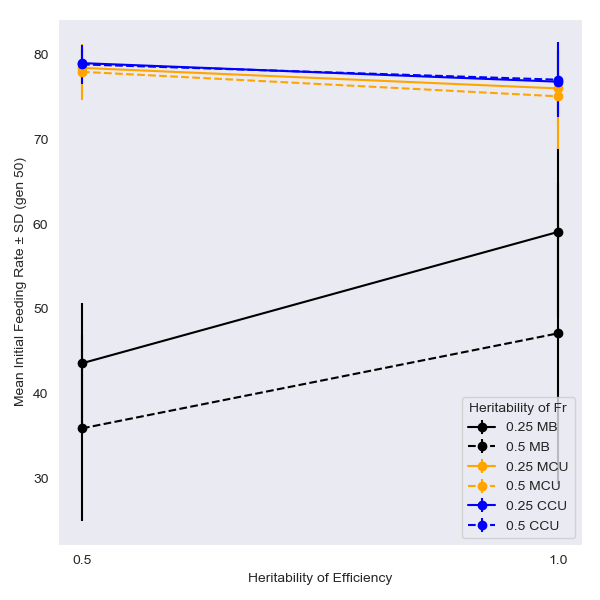
\includegraphics[width=0.5\textwidth]{C5/Figs/hrt/fr_eff_fr50}
  }
  \subfloat{
  \centering
  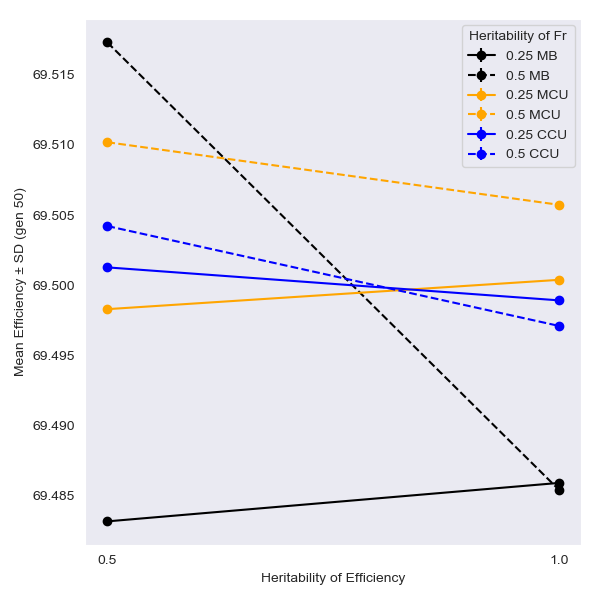
\includegraphics[width=0.5\textwidth]{C5/Figs/hrt/fr_eff_eff50}
  }\\
  \subfloat{
  \centering
  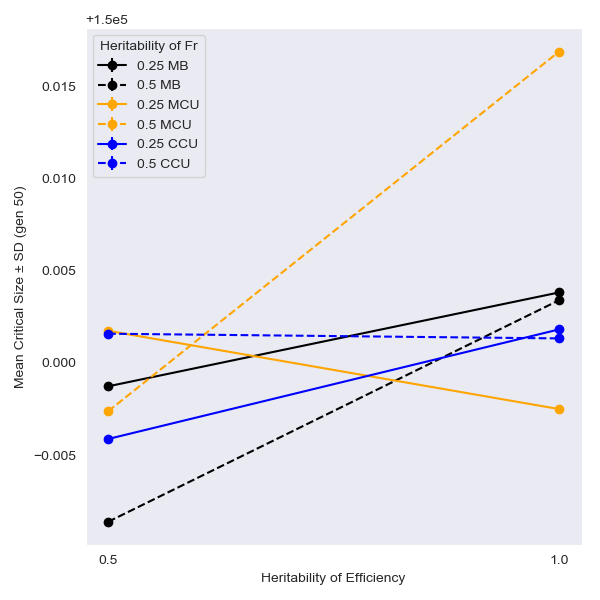
\includegraphics[width=0.5\textwidth]{C5/Figs/hrt/fr_eff_mc50}
  }
  \subfloat{
  \centering
  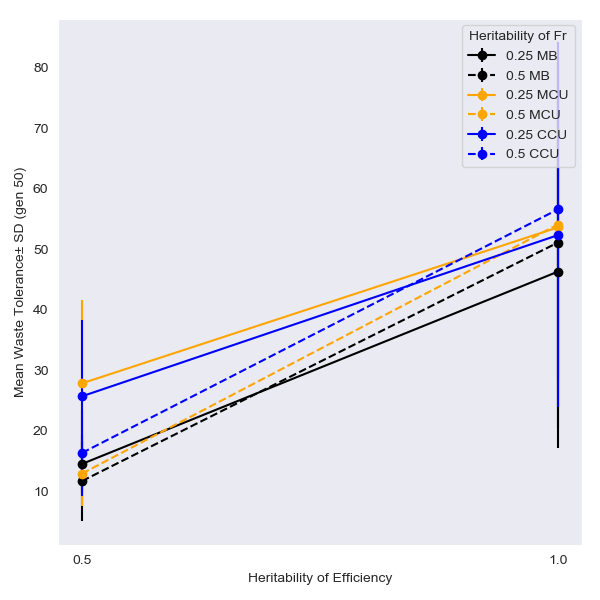
\includegraphics[width=0.5\textwidth]{C5/Figs/hrt/fr_eff_wtol50}
  }
  \caption{Effect of heritability in initial feeding rate and efficiency on mean trait values at generation 50.}
  \label{fig:hrt_fr_eff}
\end{figure}
\begin{figure}[p]
  \subfloat{
  \centering
  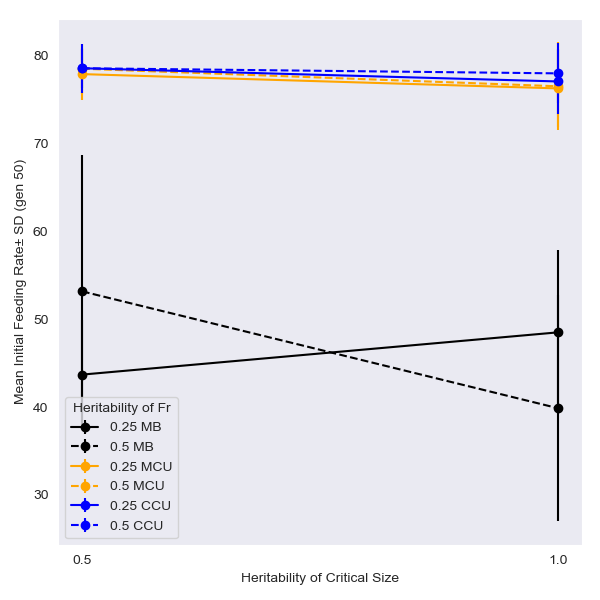
\includegraphics[width=0.5\textwidth]{C5/Figs/hrt/fr_mc_fr50}
  }
  \subfloat{
  \centering
  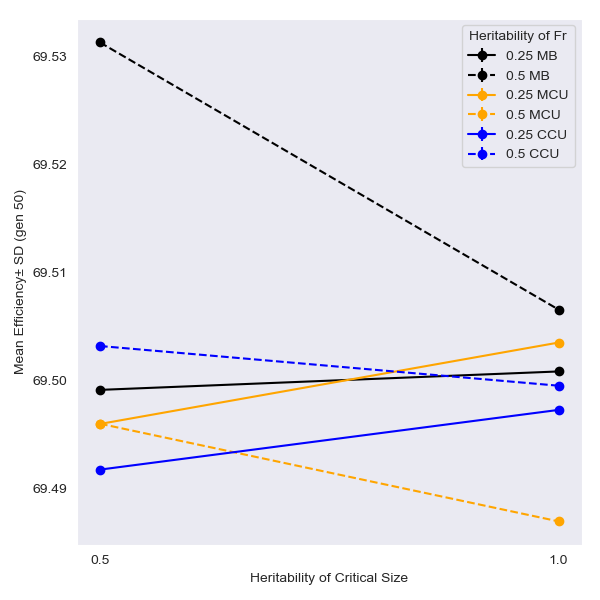
\includegraphics[width=0.5\textwidth]{C5/Figs/hrt/fr_mc_eff50}
  }\\
  \subfloat{
  \centering
  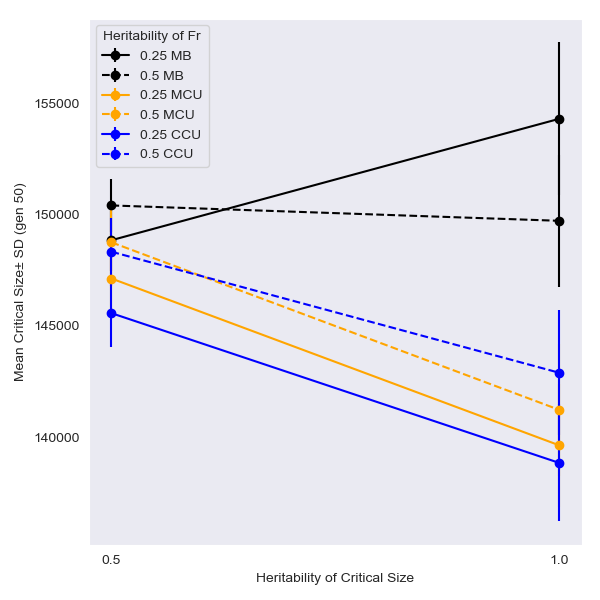
\includegraphics[width=0.5\textwidth]{C5/Figs/hrt/fr_mc_mc50}
  }
  \subfloat{
  \centering
  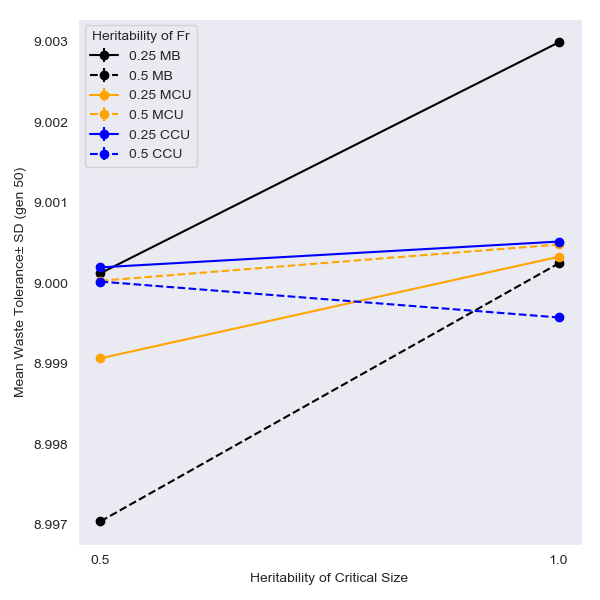
\includegraphics[width=0.5\textwidth]{C5/Figs/hrt/fr_mc_wtol50}
  }
  \caption{Effect of heritability in initial feeding rate and critical size on mean trait values at generation 50.}
  \label{fig:hrt_fr_mc}
\end{figure}
\begin{figure}[p]
  \subfloat{
  \centering
  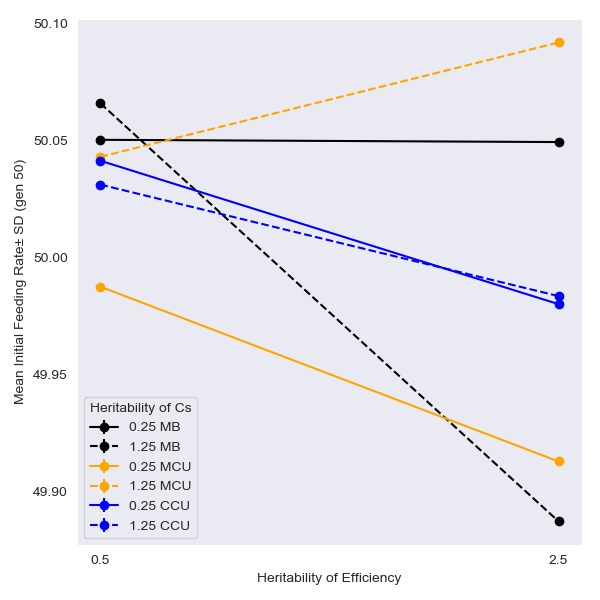
\includegraphics[width=0.5\textwidth]{C5/Figs/hrt/mc_eff_fr50}
  }
  \subfloat{
  \centering
  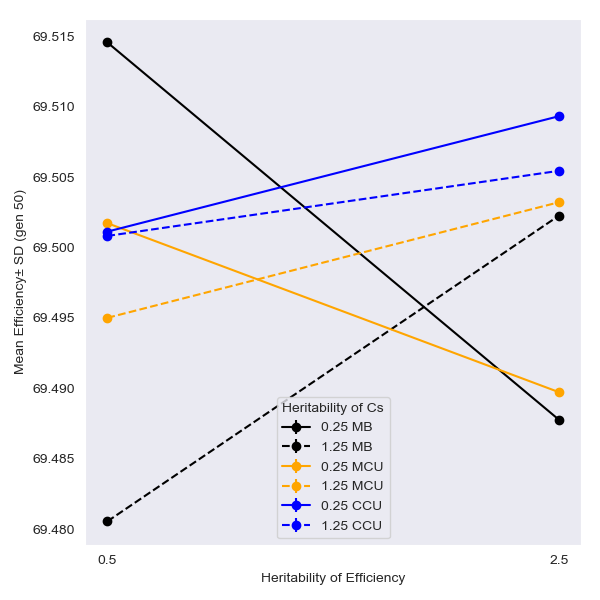
\includegraphics[width=0.5\textwidth]{C5/Figs/hrt/mc_eff_eff50}
  }\\
  \subfloat{
  \centering
  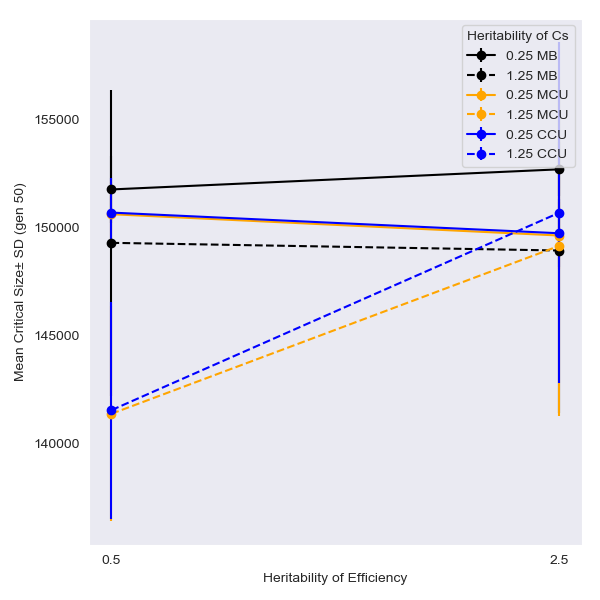
\includegraphics[width=0.5\textwidth]{C5/Figs/hrt/mc_eff_mc50}
  }
  \subfloat{
  \centering
  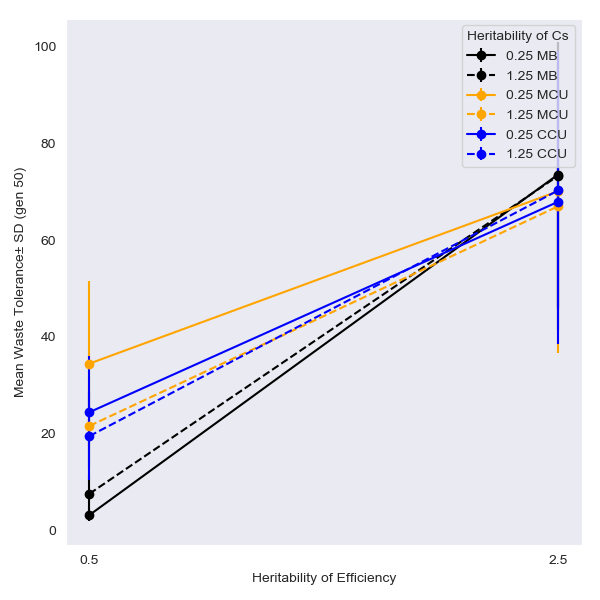
\includegraphics[width=0.5\textwidth]{C5/Figs/hrt/mc_eff_wtol50}
  }
  \caption{Effect of heritability in critical size and efficiency on mean trait values at generation 50.}
  \label{fig:hrt_mc_eff}
\end{figure}
\pagebreak
